  \begin{frame}{Aufgabe 1: Rauschanalyse}
    \begin{figure}
      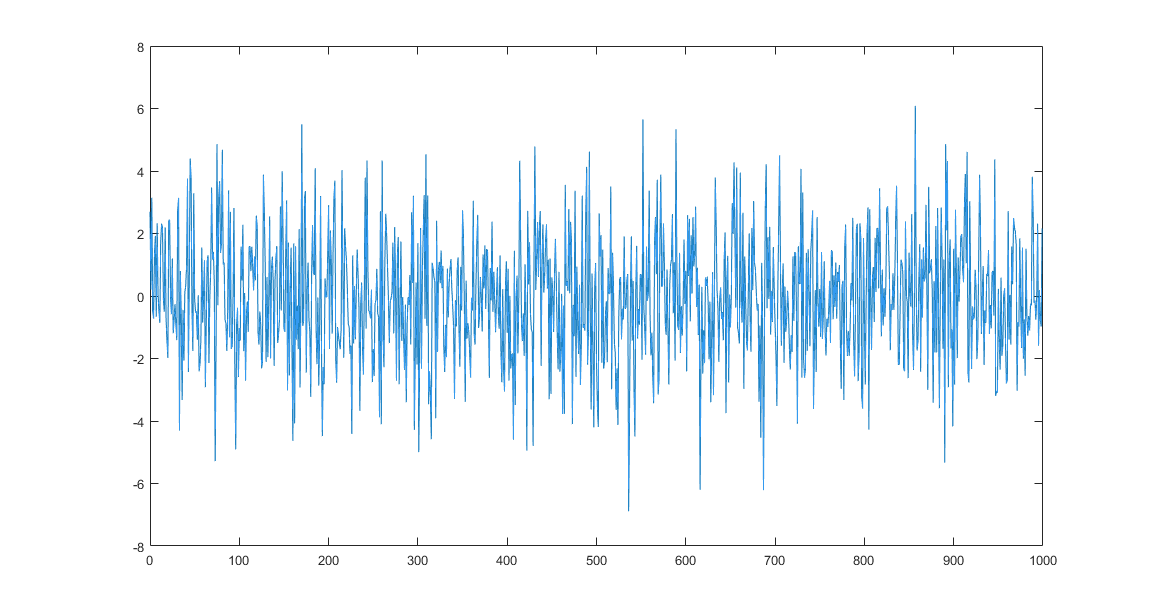
\includegraphics[width=\textwidth]{screenshots/Aufgabe1/Aufgabe1_plot}
    \end{figure}
  \end{frame}

  \begin{frame}{Aufgabe 1: Rauschanalyse}

    \twocolumns{
      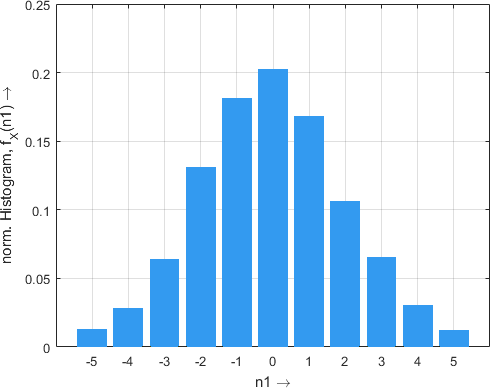
\includegraphics[width=\textwidth]{screenshots/Aufgabe1/histogram_n1}
    } {
      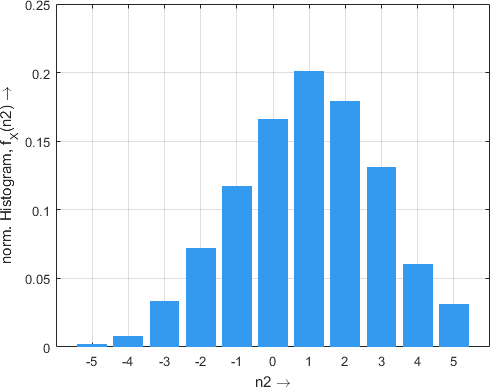
\includegraphics[width=\textwidth]{screenshots/Aufgabe1/histogram_n2}
    } {0.5\textwidth}
    
  \end{frame}

  \begin{frame}[fragile]{Aufgabe 1: Rauschanalyse}
    \begin{lstlisting}
      ...
      xmue1 = mean(n1)
      var1  = var(n1)
      ...
      \end{lstlisting}


      \begin{table}[H]
        \begin{tabular}{
          >{\columncolor{gray0}}l ll}
          Signal & \cellcolor{gray0}Mittelwert & \cellcolor{gray0}Varianz \\
          $n_1(t)$ &  $-0.06$                            & $4.00$                              \\
          $n_2(t)$    &  $0.96$                              &            $3.94$                 
        \end{tabular}
      \end{table}
      
  \end{frame}
